\documentclass[journal,12pt,twocolumn]{IEEEtran}

\usepackage{setspace}
\usepackage{gensymb}

\singlespacing


\usepackage[cmex10]{amsmath}

\usepackage{amsthm}

\usepackage{mathrsfs}
\usepackage{txfonts}
\usepackage{stfloats}
\usepackage{bm}
\usepackage{cite}
\usepackage{cases}
\usepackage{subfig}

\usepackage{longtable}
\usepackage{multirow}

\usepackage{enumitem}
\usepackage{mathtools}
\usepackage{steinmetz}
\usepackage{tikz}
\usepackage{circuitikz}
\usepackage{verbatim}
%\usepackage{tfrupee}
\usepackage[breaklinks=true]{hyperref}
\usepackage{graphicx}
\usepackage{tkz-euclide}
\usepackage{float}

\usetikzlibrary{calc,math}
\usepackage{listings}
    \usepackage{color}                                            %%
    \usepackage{array}                                            %%
    \usepackage{longtable}                                        %%
    \usepackage{calc}                                             %%
    \usepackage{multirow}                                         %%
    \usepackage{hhline}                                           %%
    \usepackage{ifthen}                                           %%
    \usepackage{lscape}     
\usepackage{multicol}
\usepackage{chngcntr}

\DeclareMathOperator*{\Res}{Res}

\renewcommand\thesection{\arabic{section}}
\renewcommand\thesubsection{\thesection.\arabic{subsection}}
\renewcommand\thesubsubsection{\thesubsection.\arabic{subsubsection}}

\renewcommand\thesectiondis{\arabic{section}}
\renewcommand\thesubsectiondis{\thesectiondis.\arabic{subsection}}
\renewcommand\thesubsubsectiondis{\thesubsectiondis.\arabic{subsubsection}}


\hyphenation{op-tical net-works semi-conduc-tor}
\def\inputGnumericTable{}                                 %%

\lstset{
%language=C,
frame=single, 
breaklines=true,
columns=fullflexible
}
\begin{document}
\newtheorem{theorem}{Theorem}[section]
\newtheorem{problem}{Problem}
\newtheorem{proposition}{Proposition}[section]
\newtheorem{lemma}{Lemma}[section]
\newtheorem{corollary}[theorem]{Corollary}
\newtheorem{example}{Example}[section]
\newtheorem{definition}[problem]{Definition}

\newcommand{\BEQA}{\begin{eqnarray}}
\newcommand{\EEQA}{\end{eqnarray}}
\newcommand{\define}{\stackrel{\triangle}{=}}
\bibliographystyle{IEEEtran}
\providecommand{\mbf}{\mathbf}
\providecommand{\pr}[1]{\ensuremath{\Pr\left(#1\right)}}
\providecommand{\qfunc}[1]{\ensuremath{Q\left(#1\right)}}
\providecommand{\sbrak}[1]{\ensuremath{{}\left[#1\right]}}
\providecommand{\lsbrak}[1]{\ensuremath{{}\left[#1\right.}}
\providecommand{\rsbrak}[1]{\ensuremath{{}\left.#1\right]}}
\providecommand{\brak}[1]{\ensuremath{\left(#1\right)}}
\providecommand{\lbrak}[1]{\ensuremath{\left(#1\right.}}
\providecommand{\rbrak}[1]{\ensuremath{\left.#1\right)}}
\providecommand{\cbrak}[1]{\ensuremath{\left\{#1\right\}}}
\providecommand{\lcbrak}[1]{\ensuremath{\left\{#1\right.}}
\providecommand{\rcbrak}[1]{\ensuremath{\left.#1\right\}}}
\theoremstyle{remark}
\newtheorem{rem}{Remark}
\newcommand{\sgn}{\mathop{\mathrm{sgn}}}
\providecommand{\abs}[1]{\vert#1\vert}
\providecommand{\res}[1]{\Res\displaylimits_{#1}} 
\providecommand{\norm}[1]{\lVert#1\rVert}
%\providecommand{\norm}[1]{\lVert#1\rVert}
\providecommand{\mtx}[1]{\mathbf{#1}}
\providecommand{\mean}[1]{E[ #1 ]}
\providecommand{\fourier}{\overset{\mathcal{F}}{ \rightleftharpoons}}
%\providecommand{\hilbert}{\overset{\mathcal{H}}{ \rightleftharpoons}}
\providecommand{\system}{\overset{\mathcal{H}}{ \longleftrightarrow}}
	%\newcommand{\solution}[2]{\textbf{Solution:}{#1}}
\newcommand{\solution}{\noindent \textbf{Solution: }}
\newcommand{\cosec}{\,\text{cosec}\,}
\providecommand{\dec}[2]{\ensuremath{\overset{#1}{\underset{#2}{\gtrless}}}}
\newcommand{\myvec}[1]{\ensuremath{\begin{pmatrix}#1\end{pmatrix}}}
\newcommand{\mydet}[1]{\ensuremath{\begin{vmatrix}#1\end{vmatrix}}}
\numberwithin{equation}{subsection}
\makeatletter
\@addtoreset{figure}{problem}
\makeatother
\let\StandardTheFigure\thefigure
\let\vec\mathbf
\renewcommand{\thefigure}{\theproblem}
\def\putbox#1#2#3{\makebox[0in][l]{\makebox[#1][l]{}\raisebox{\baselineskip}[0in][0in]{\raisebox{#2}[0in][0in]{#3}}}}
     \def\rightbox#1{\makebox[0in][r]{#1}}
     \def\centbox#1{\makebox[0in]{#1}}
     \def\topbox#1{\raisebox{-\baselineskip}[0in][0in]{#1}}
     \def\midbox#1{\raisebox{-0.5\baselineskip}[0in][0in]{#1}}
\vspace{3cm}
\title{ASSIGNMENT 5}
\author{Dishank Jain \\ AI20BTECH11011}
\maketitle
\newpage
\bigskip
\renewcommand{\thefigure}{\theenumi}
\renewcommand{\thetable}{\theenumi}
Download all python codes from
%
\begin{lstlisting}
https://github.com/Dishank422/EE3900/blob/main/assignment5/codes
\end{lstlisting}
% 
and latex-tikz codes from 
%
\begin{lstlisting}
https://github.com/Dishank422/EE3900/blob/main/assignment5/Assignment5.tex
\end{lstlisting}
%
\section{Quadratic forms Q 2.68}
Find the normal at the point $\myvec{1\\1}$ on the curve $2y+x^2=3$.

\section{Solution}
The given curve can be expressed as 
\begin{align}
    &x^2+2y-3=0\\
    \implies \vec{V} = &\myvec{1&0\\0&0},\; \vec{u} = \myvec{0\\1},\; \vec{f} = -3
\end{align}

Since $\abs{\vec{V}} = 0$, the given curve represents a parabola. The eigenvalues are given by 
\begin{equation}
    \lambda_1 = 0, \; \lambda_2 = 1
\end{equation}

with corresponding eigenvectors 
\begin{align}
    \myvec{1&0\\0&0}\vec{x} = 0 \implies \vec{p}_1 = \myvec{0\\1}\\
    \myvec{0&0\\0&-1}\vec{x} = 0 \implies \vec{p}_2 = \myvec{1\\0}
\end{align}

To find the vertex of the parabola,
\begin{equation}
    \myvec{\vec{u}^\top+\kappa \vec{p}_1^\top\\\vec{V}}\vec{c} = \myvec{-\vec{f}\\\kappa \vec{p}_1-\vec{u}}
\end{equation}

where, $\kappa = \vec{u}^\top\vec{p}_1 = 1$
\begin{align}
    \implies \myvec{0&2\\1&0\\0&0}\vec{c} &= \myvec{3\\0\\0}\\
    \implies \vec{c} &= \myvec{0\\1.5}
\end{align}

Now to evaluate the direction vector $\vec{m}$,
\begin{align}
    \vec{m}^\top (\vec{V}\vec{q}+\vec{u}) &= 0\\
    \implies \vec{m}^\top \myvec{\myvec{1&0\\0&0}\myvec{1\\1}+\myvec{0\\1}} &= 0\\
    \implies \vec{m}^\top \myvec{1\\1} &= 0\\
    \implies \vec{m} &= \myvec{-1\\1}
\end{align}

The normal is obtained as 
\begin{align}
    \vec{m}^\top (\vec{x}-\vec{q}) &= 0\\
    \implies \myvec{-1&1}\myvec{\vec{x}-\myvec{1\\1}} &= 0\\
    \implies \myvec{-1&1}\vec{x} &= 0
\end{align}

The above results are verified in Fig. \ref{plot}. 
\begin{figure}
    \centering
    \resizebox{\columnwidth}{!}{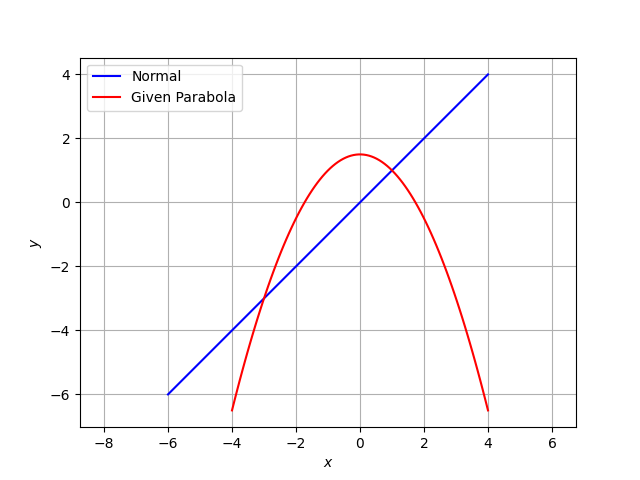
\includegraphics{figures/figure.png}}
    \caption{Plot of the normal}
    \label{plot}
\end{figure}
\end{document}
